
\subsection{Ikeda's original method: a strip theory based method}
\label{se:semi-empirical methods}

The roll damping consists of linear and nonlinear components. At zero speed the nonlinear damping is caused by the two-dimensional separation at the bilge keel or near the bilge circle (Eddy damping $B_E$). While at speed the nonlinear damping is mainly caused by the hydrodynamic lift force on the hull, represented as lift damping $B_L$. $B_E$ vanishes at high speed ($F_n>0.15)$ \cite{ikeda_components_1978}.

The wave damping also changes at speed. Ikeda \cite{ikeda_components_1978} proposes a formula for the fraction between wave damping at speed and zero speed: $\frac{B_W}{B_{W0}}$

The Ikeda method has been used to calculate the roll damping for a PCTC vessel Faust \cite{soder_assessment_2019}.


%\begin{figure}[h]
%    \centering
%    \includegraphics[width=\columnwidth]{figures/ikeda_faust.pdf}
%    \caption{Roll damping components calculated with Ikeda method for PCTC Faust}
%    \label{fig:ikeda_faust}
%\end{figure}



The Ikeda method \cite{ikeda_roll_1978}, \cite{ikeda_eddy_1978}, \cite{ikeda_roll_1979}, \cite{ikeda_components_1978}, \cite{ikeda_velocity_1979} is the most well known semi empirical method to predict roll damping. 

\begin{equation} \label{eq:ikeda}
B = B_F + B_E + B_L + B_W + B_{BK}
\end{equation}

This method divides the roll damping into friction, eddy, lift, waves and bilge keel components (see equation \ref{eq:ikeda}. The wave and eddy components require strip method calculations. This is not an attractive option for the present study since that would require calculations with exact hull geometries to be carried out for all of the ships in the study. There exist however a \emph{Simplified Ikeda method} \cite{kawahara_simple_2011} that is instead used in this study to calculate the eddy component $B_E$ and wave component $B_W$. Figure \ref{fig:ikeda_vs_simplified} shows a comparison between roll damping components calculated with \emph{Ikeda} and \emph{Simplified Ikeda method}. The roll damping is under-predicted with the simplified method for this particular case which is expected according to the limitations of this method  \cite{kawahara_simple_2011}.

\begin{figure}[h]
    \centering
    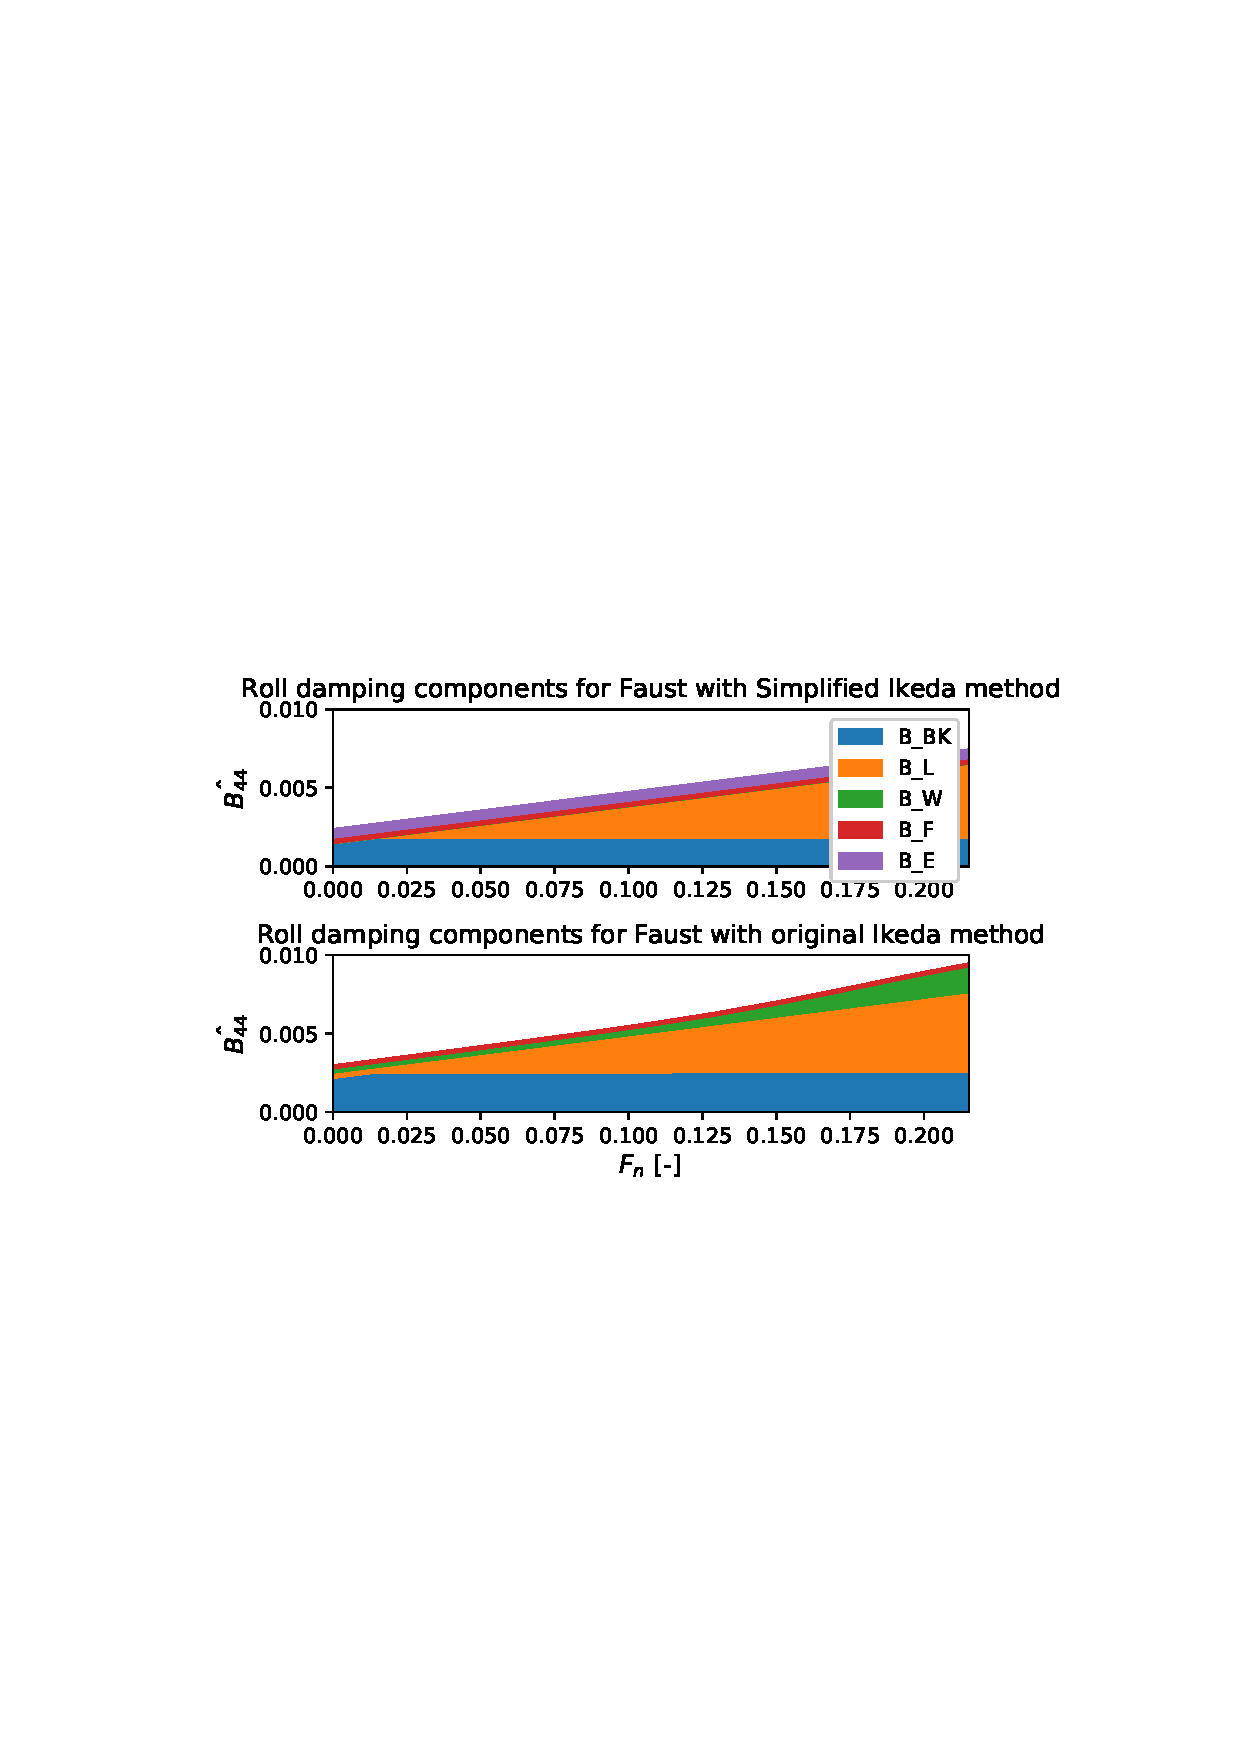
\includegraphics[height=7cm, width=14cm]{figures/ikeda_vs_simplified.pdf}
    \caption{Roll damping components calculated with Ikeda and Simplified Ikeda for PCTC Faust}
    \label{fig:ikeda_vs_simplified}
\end{figure}
